\section{Classification \& Bio-geophysical Parameter Retrieval}

\subsection{Can we predict where there is chlorophyll through classification?}

We will use \textit{K-Means clustering} to classify the data. K-means clustering is a 
unsupervised learning algorithm that can be used to classify and cluster data into $k$ 
different clusters. The data points are adjusted iteratively until all points are 
associated with the nearest cluster.

We want to cluster each observation (pixels, with $n$ spectral channels) into a specific 
cluster (environment class, ie. deep water, shallow water, vegetation). 

As we can see from \cref{fig:point_spectra}, we know that those three different points 
have distinctly different spectra, thus it should be possible to classify them accordingly. 

\begin{figure}
    \centering
    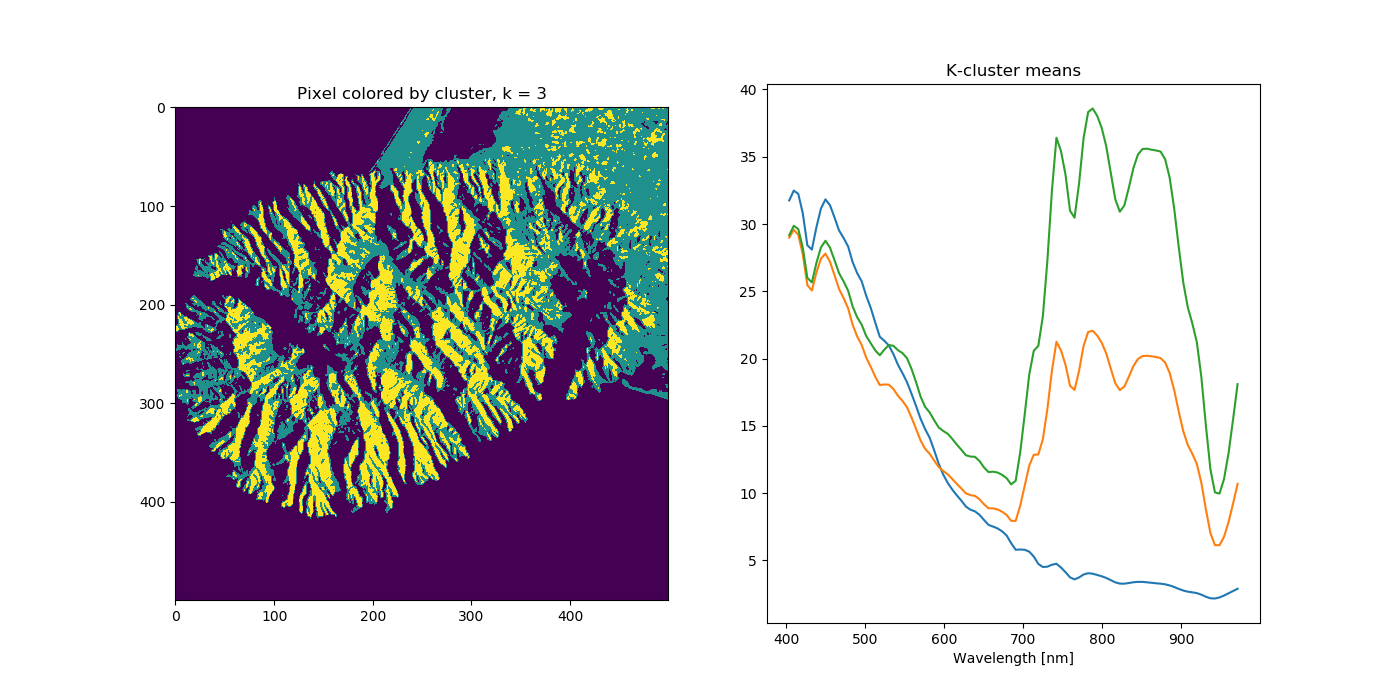
\includegraphics[width=\textwidth]{../fig/kmean/kmean_3.png}
    \caption{K-mean clusters of the image}
    \label{fig:kmean}
\end{figure}


\subsection{How well can we directly estimate the chlorophyll content?}

\subsection{How can we estimate the reflectance from the surface of the ocean?}

\subsection{Compute chlorophyll concentration using atmosphere-corrected data}

\subsection{Classify land versus water}

\subsection{Other bio-geophysical parameters}

\subsection{Alternative atmospheric correction methods}